\section{Background and Preliminaries}

% \zxh{Rewrite this entire section, clearly and formally.}
This section establishes the empirical and conceptual basis for our
autonomy-centered view of recursive self-improvement.
We first examine the uneven progress of modern foundation models across
different capability domains, highlighting why persistent improvement is
particularly relevant to interactive, stateful, and tool-using systems.
We then characterize RSI through the structure of an improvement loop,
introduce the key components needed to analyze how improvements are generated,
validated, retained, and inherited, and distinguish RSI from neighboring
paradigms such as continual learning, AutoML, and agentic AI.
Finally, because contemporary RSI spans both academic research and industrial
engineering practice, we clarify the scope and strength of the evidence used
throughout this survey.
Together, these preliminaries provide the empirical motivation, operational
vocabulary, and evidentiary basis for the autonomy hierarchy developed in the
following section.

% This section covers historical context, definitions, related concepts, and the evidence scope. It briefly traces self-modifying programs, the G\"odel Machine, AutoML, continual learning, agentic AI, modern RSI, and prospective ASI.

% Our operational definition emphasizes persistent updates, effects on subsequent tasks, and a closed improvement loop.

% \subsection{Boundary Cases}
% Distinguish the following from strict system self-improvement:
% \begin{itemize}
%   \item one-off reflection and output revision;
%   \item test-time search;
%   \item ordinary workflow automation;
%   \item improvement of external scientific artifacts; and
%   \item human-led continual training.
% \end{itemize}

% \subsection{Evidence Scope}
% State inclusion criteria for papers, technical reports, official blogs, open-source projects, and company materials, together with the differing strength of evidence supplied by each source type.

\subsection{Uneven Capability Progress in Modern Foundation Models}

\begin{figure*}[!t]
    \centering
    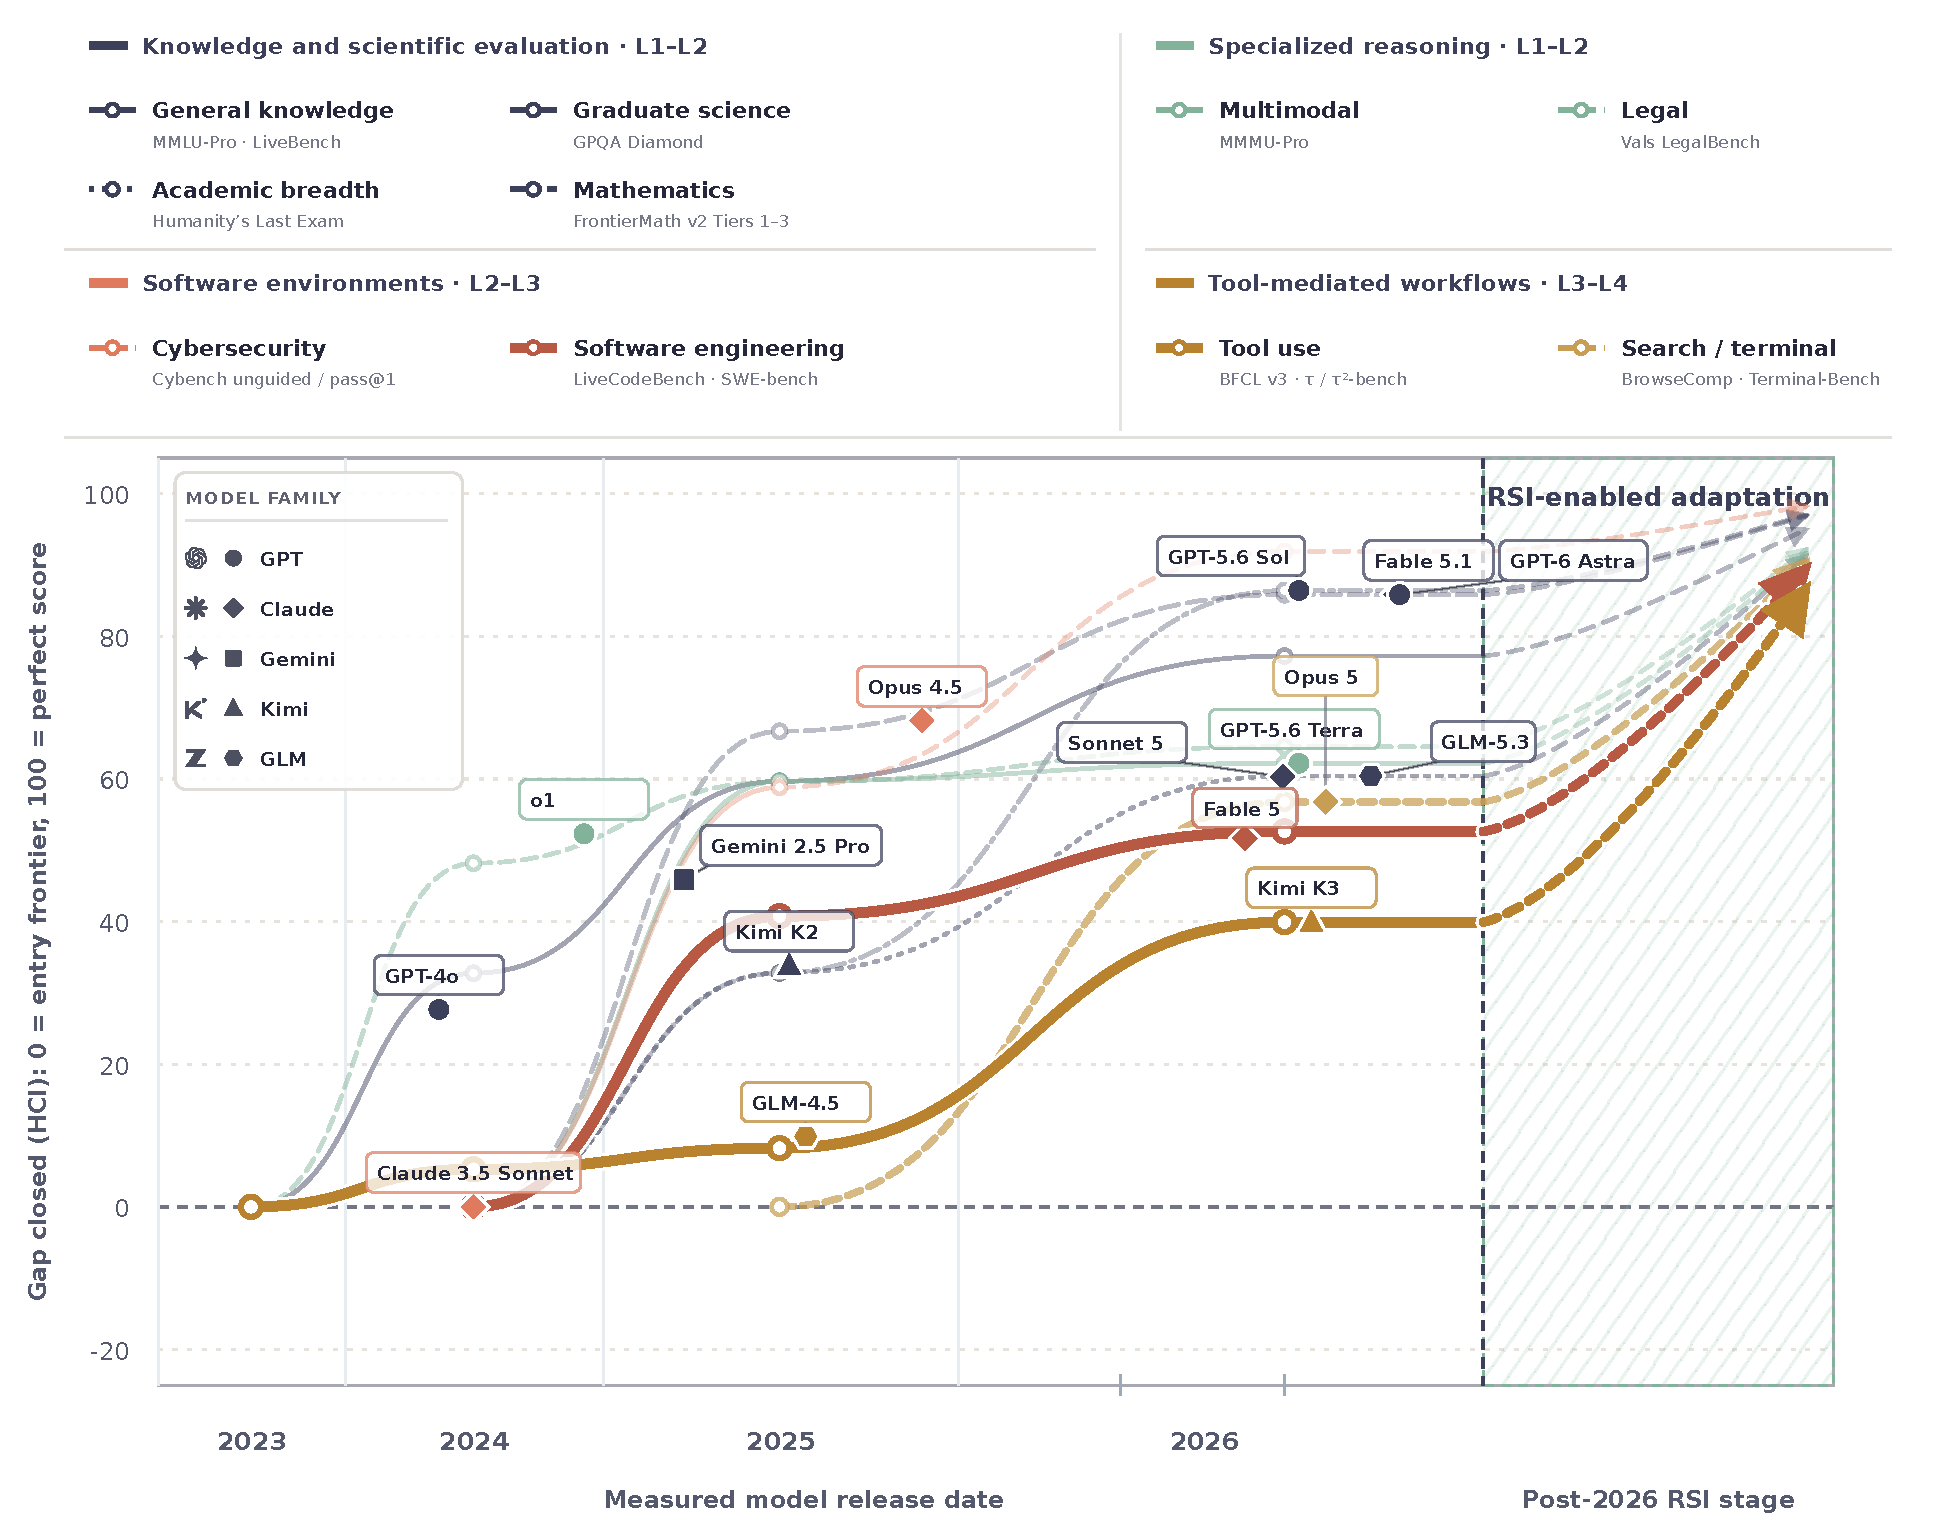
\includegraphics[width=\textwidth]{figures/RSI_Longitudinal_Capability_Plot_v0.21.pdf}
    \caption{Cross-domain capability trajectories and an illustrative RSI extension. Each line reports an annual domain frontier in HCI, where 0 is the benchmark's entry-year frontier and 100 is a perfect score. Dashed cybersecurity segments denote changes in Cybench subsets or \texttt{pass@1} aggregation. The post-2026 region illustrates the extension of domains with the assistance of RSI.}
    \label{fig:rsi-longitudinal-capability}
\end{figure*}

Figure~\ref{fig:rsi-longitudinal-capability} summarizes 393 eligible model--benchmark observations across ten capability domains for models released between 2023 and September 2026.

We first group reported scores into protocol-link families. Two results belong to the same family only when the benchmark version and evaluation harness remain stable, or when evaluations of overlapping models provide a defensible bridge between protocols. Results obtained with incompatible versions or harnesses remain in the audit records but are excluded from the trajectories. This rule admitted 17 of the 33 results considered in the latest-model audit. The other 16, drawn from Terminal-Bench~\cite{merrill2026terminalbench}, DeepSWE~\cite{huang2026deepswe}, CyberGym~\cite{wang2025cybergym}, ExploitBench~\cite{lee2026exploitbench}, AutomationBench~\cite{shepard2026automationbench}, and BrowseComp~\cite{wei2025browsecomp}, were retained for reference because their benchmark versions or evaluation settings could not be linked to the plotted families. If several sources report the same model under the same benchmark family, variant, and evaluation mode, we calculate the following weighted consensus:
\begin{equation}
\bar{s}_{mbh}=\frac{\sum_i \widetilde{w}_i s_{imbh}}{\sum_i \widetilde{w}_i},
\label{eq:source-weighted-consensus}
\end{equation}
where $h$ denotes the evaluation protocol and $i$ indexes sources. Benchmark-owner tables, independent common-harness evaluations, combined benchmark or model reports, and model-author tables receive base weights of 3, 2.5, 2, and 1, respectively. We multiply first-party values by an additional factor of 0.75. These weights provide a practical sensitivity adjustment, limiting the influence of self-reported results.

The underlying benchmarks report different quantities, so their raw values cannot be pooled directly. We normalize the consensus score with the Headroom-Closed Index (HCI). For model $m$ on benchmark family $b$ under protocol $h$,
\begin{equation}
H_{mbh}=100\times\frac{\bar{s}_{mbh}-F_{b,0}}{100-F_{b,0}},
\label{eq:headroom-closed-index}
\end{equation}
where $F_{b,0}$ is the 90th-percentile model score in the first year that benchmark enters the dataset. Thus, $H_{mbh}=0$ denotes the entry-year frontier and $H_{mbh}=100$ denotes a perfect score. For each benchmark family and release year, we first compute the 90th-percentile HCI frontier $Q_{b,y}$. The domain trajectory is then
\begin{equation}
T_{d,y}=\frac{\sum_{b\in\mathcal{B}_{d,y}}\sqrt{n_{b,y}}\,Q_{b,y}}
{\sum_{b\in\mathcal{B}_{d,y}}\sqrt{n_{b,y}}},
\label{eq:domain-hci-trajectory}
\end{equation}
where $\mathcal{B}_{d,y}$ is the set of eligible benchmark families for domain $d$ in year $y$, and $n_{b,y}$ is the number of distinct models contributing to that benchmark-year frontier. The square-root weight allows better-covered families to contribute more without letting the largest table dominate the domain value. Three observations follow.

\noindent$\bullet$ \bfit{Observation 1: Frontier gains differ in magnitude and timing.}
By 2026, advanced mathematics and graduate-level science reach HCI values of 86.4 and 85.8, while broad knowledge reaches 77.2. The corresponding values for legal reasoning, multimodal reasoning, and frontier academic breadth are 64.5, 62.2, and 60.4. The annual increment $\Delta T_{d,y}=T_{d,y}-T_{d,y-1}$ exposes different temporal patterns. Broad knowledge rises by 32.8, 26.9, and 17.6 points across the three annual transitions, indicating steady but slowing headroom closure. Legal reasoning similarly slows from a 48.2-point gain in 2024 to 11.4 in 2025 and 4.9 in 2026. Advanced mathematics follows a different path, whose increment grows from 32.8 points in 2025 to 53.6 in 2026. Multimodal reasoning gains 59.7 points in 2025 but only 2.5 in 2026. A single aggregate benchmark would conceal these differences in both level and trajectory shape.

\noindent$\bullet$ \bfit{Observation 2: Interactive capabilities retain larger gaps.}
Software engineering reaches an HCI of 52.6 in 2026, search and terminal agents reach 56.8, and tool agents reach 39.9. Relative to graduate-level science at 85.8, their normalized headroom closure is lower by 33.2, 29.1, and 45.9 points, respectively. Tool agents improve sharply in 2026, from 8.2 to 39.9, yet remain the lowest trajectory. Software engineering gains 40.8 points in 2025 and 11.9 in 2026. The leading cybersecurity-agent trajectory reaches 91.9, producing a 52.0-point difference from tool agents. This comparison requires caution because the later Cybench observations use changed task subsets or \texttt{pass@1} aggregation, as indicated by the dashed line. Even with that qualification, the figure shows that gains in bounded or readily verified environments have not transferred uniformly to long, stateful workflows. Model developers increasingly turned their attention to agentic coding and tool use after 2024, and these capabilities became prominent research and engineering targets during 2025 and 2026~\cite{wang2026hgm,chen2026sweexp,sun2026seagent,li2026pando}. Such tasks require planning, environment-state tracking, tool selection, result interpretation, and revision of subsequent actions. Errors propagate across the trajectory, so data collection and evaluation must cover complete interactions. In the paper's autonomy taxonomy, bounded evaluations mainly exercise L1--L2 capabilities, environment tasks increasingly require L2--L3 capabilities, and interactive workflows expose the verification, memory, and adaptation requirements associated with L3--L4 operation.

\noindent$\bullet$ \bfit{Observation 3: Remaining headroom concentrates the potential value of RSI.}
The hatched post-2026 region illustrates how persistent and verified recursive self-improvement could preferentially affect domains with larger remaining gaps. To express this relationship consistently, the illustrative endpoint for domain $d$ is
\begin{equation}
R_d=100-0.22\left(100-T_{d,2026}\right).
\end{equation}
Equivalently, the illustrative gain is $R_d-T_{d,2026}=0.78(100-T_{d,2026})$, so domains with more unclosed headroom receive a larger extension. Cybersecurity therefore moves from 91.9 to 98.2, while software engineering, search and terminal agents, and tool agents move from 52.6 to 89.6, from 56.8 to 90.5, and from 39.9 to 86.8. The endpoints illustrate the hypothesis that repeated experience generation, validation, update retention, and regression testing could direct more improvement toward weak deployment workflows.

Software engineering and tool use are therefore particularly relevant to RSI. Human-led updates require repeated environment construction, trajectory collection, failure diagnosis, training or harness revision, and regression testing as interfaces and repositories change. The methods reviewed later generate practice from observed weaknesses~\cite{sun2026seagent}, distill trajectories into reusable rules and tools~\cite{li2026pando,dai2026metis}, and retain tested harness or code changes for future tasks~\cite{zhang2026selfharness,lin2026ahe}. These mechanisms can direct successive updates toward failures observed during deployment and reduce the capability gaps represented by the illustrative extensions.

\subsection{Conceptual Foundations of Recursive Self-Improvement}

The idea that an intelligent system may participate in improving its own future behavior has several intellectual predecessors, including self-modifying programs, the G\"odel Machine, automated machine learning, meta-learning, continual learning, open-ended learning, and more recent agentic systems capable of modifying code, prompts, tools, or training procedures~\cite{schmidhuber2003godel,ye2026ai4ai,shi2025continual,wang2019poet,hu2025adas,zhang2025aflow}. These traditions address overlapping parts of the problem, but they do not by themselves provide a sufficient criterion for \RSI. Automated optimization does not necessarily imply self-improvement, persistent learning does not necessarily imply autonomy over the learning process, and an AI-generated improvement to an external artifact does not necessarily modify the AI system that generated it.

For this reason, we take the \emph{improvement loop} rather than any particular algorithm as the basic unit of analysis. This perspective allows systems implemented through very different mechanisms to be compared according to the same questions: what generates the experience, what is changed, what persists into future interactions, who controls the update process, and whether the result of one improvement round participates in determining subsequent improvements.



\subsubsection{Anatomy of an Improvement Loop}

\noindent\bfit{Improvement loop.}
We define an improvement loop as a recurring process in which an AI system uses experience to propose a modification to a target, evaluates the candidate under an acceptance rule, retains an accepted change in its state, and begins the next round from that updated state. The following components identify where each operation occurs and what information passes between rounds.

\noindent$\bullet$ \bfit{AI system:} the complete computational entity whose capability state is tracked across improvement cycles. It includes the mechanisms and persistent state that determine how the system acts, generates modifications from feedback, and carries accepted results into the next round. In automated code improvement, for example, the AI system includes the components that propose a patch, execute the modified program, evaluate the result, and continue from a retained version.

\noindent$\bullet$ \bfit{System state:} the part of the AI system retained at the end of one round and inherited by the next. It is what the next round receives from the previous one. If a system accepts a faster program and continues modifying that version, the retained program belongs to its system state.

\noindent$\bullet$ \bfit{Experience:} information obtained from earlier interactions and used to guide a later modification. A test failure, environment outcome, or reviewer correction becomes experience when it informs a subsequent update.

\noindent$\bullet$ \bfit{Target:} the object directly modified in the current round. In code optimization, the target may be a sorting function. If the system later changes its method for generating code candidates, that search method becomes the target.

\noindent$\bullet$ \bfit{Improver:} % the system requires a mechanism for \emph{evaluation and selection}
the mechanism that transforms the current state and available experience into candidate modifications. A model that reads the current code and a recent test failure before proposing the next patch acts as the improver in that round.

\noindent$\bullet$ \bfit{Strategy:} the method used by the improver to decide where to search and how to generate candidates. A strategy may prioritize code locations implicated in failed tests. Because the strategy can be retained, it may also become a target of later improvement.

\noindent$\bullet$ \bfit{Verifier:} the mechanism that evaluates candidates and applies the acceptance rule. It may use benchmark scores, unit tests, reward models, environment outcomes, human feedback, formal constraints, safety checks, or combinations of these signals.

\noindent$\bullet$ \bfit{Improvement:} a candidate modification that passes the current acceptance rule, is retained, and enters the next system state. An improvement is therefore an accepted and inherited state change.

% \emph{Successor}: an accepted update must be \emph{persisted and re-enter the system's future operation}. This is the point at which an improvement loop differs from an isolated optimization episode. 

% \emph{Update Path}

% \emph{Interaction history or source of experience}
\noindent$\bullet$ \bfit{Successor:} the AI system that inherits one or more accepted improvements and enters the next round with an updated state. For example, a system that retains a revised code-search strategy and uses it to generate later modifications is the successor of the version that produced the strategy.

This decomposition yields three cross-cutting questions that will be used throughout the survey. \emph{Where does the loop close?} determines whether an apparent improvement actually returns to the system. \emph{What is updated and inherited?} determines the persistent carrier of improvement. \emph{Which decisions remain external?} determines how much authority over the improvement process has been transferred from humans or fixed infrastructure to the AI system itself.

This anatomy applies to persistent improvement processes with different degrees of automation. The next subsection specifies the additional conditions for \RSI{}: experience must produce persistent self-change with sufficient autonomy, and an accepted change must be able to affect how later improvements are generated, evaluated, selected, or consolidated.

\subsubsection{Definition of Recursive Self-Improvement}
Using the improvement-loop anatomy above, we define \emph{recursive self-improvement} (\RSI) as the capability of an intelligent system, through continued interaction with tasks, environments, or other intelligent agents, to autonomously transform acquired experience and feedback into persistent changes to itself across interaction rounds (e.g., model parameters, agent harnesses, or improvement policies), such that these changes can further affect the mechanisms used to generate, evaluate, select, and consolidate subsequent self-improvements. The improved system is consequently reintroduced into the next round of interaction and improvement with an already changed capability state, allowing the system's capacity for improvement itself to become part of an ongoing recursive process.

\RSI{} contains an autonomous, closed-loop process in which AI identifies its own limitations, develops and validates improvements, and uses the resulting capabilities to improve the improvement process itself, with the aim of (1) expanding its capability frontier, (2) increasing resource efficiency, or (3) discovering novel solutions beyond human-prescribed strategies.

Recent industry perspectives increasingly operationalize \RSI\ through autonomous improvement loops. OpenAI emphasizes the automation of AI research workflows and feedback loops~\cite{openai2026rsi}, while Tencent reports an early-stage RSI loop in which experimental results are fed into subsequent rounds of model development~\cite{tencent2026hy4}. More strictly, Alibaba researchers define RSI by making the improvement mechanism itself subject to modification~\cite{liu2026path}, whereas Anthropic describes its strongest form as an AI system autonomously designing and developing its own successor~\cite{anthropic2026rsi}.

% \zxh{add industry view and academic view?}

\subsubsection{Relation to Neighboring Paradigms}
\RSI \ intersects with continual learning, automated machine learning (AutoML), and agentic AI because all three automate parts of an improvement loop. They differ in the usual target of improvement, the state retained across rounds, and the decisions left to a fixed procedure or an external actor. Table~\ref{tab:rsi-neighboring-paradigms} summarizes these distinctions.

\emph{Continual learning}: Continual learning enables a model or agent to acquire knowledge from a sequence of tasks or data while limiting the loss of earlier capabilities~\cite{shi2025continual,wu2024continual,zheng2024lifelongllms}. Recent work covers continual pre-training, instruction tuning, alignment, replay, parameter-efficient updates, and memory-based adaptation~\cite{shi2025continual,wu2024continual}. Lifelong and self-evolving agents further extend persistent state beyond model weights to memories, skills, and behavioral policies~\cite{zheng2026lifelong,fang2025selfevolving}. The learning objective, update rule, experience schedule, and acceptance test nevertheless usually remain fixed by the system designer~\cite{shi2025continual,zheng2024lifelongllms}. In our framework, continual learning approaches \RSI{} when experience can also revise how later adaptations are proposed, evaluated, or consolidated, and the revised process is reused in subsequent rounds~\cite{zheng2026lifelong,fang2025selfevolving}.

\emph{AutoML}: AutoML automates model-development decisions such as data processing, model and architecture selection, hyperparameter optimization, and pipeline construction~\cite{trirat2025automlagent,ye2026ai4ai}. Recent systems broaden this scope through language-model agents: AutoML-Agent constructs and verifies complete machine-learning pipelines, while ADAS, AFlow, and AgentSquare search over executable agent designs, workflow graphs, or reusable modules~\cite{trirat2025automlagent,hu2025adas,zhang2025aflow,shang2025agentsquare}. MLE-bench and the AI Scientist-v2 extend evaluation to sustained machine-learning engineering and iterative research workflows~\cite{chan2025mlebench,yamada2025aiscientistv2}. Their search spaces, objectives, budgets, and evaluators are generally supplied in advance, even when much of the development work is automated~\cite{trirat2025automlagent,hu2025adas,zhang2025aflow}. AutoML reaches the \RSI{} boundary when the procedure used to search for or evaluate improvements becomes persistent state that later rounds can improve~\cite{hu2025adas,zhang2025aflow,fang2025selfevolving}.

\emph{Agentic AI and agentic ML}: Agentic systems plan multistep work, invoke tools, run experiments, coordinate specialized components, and revise intermediate artifacts~\cite{chan2025mlebench,starace2025paperbench,yamada2025aiscientistv2}. MLE-bench, PaperBench, and the AI Scientist-v2 study these capabilities in machine-learning engineering and research settings~\cite{chan2025mlebench,starace2025paperbench,yamada2025aiscientistv2}, while ADAS and AFlow automate the construction of the agent or workflow that performs the task~\cite{hu2025adas,zhang2025aflow}. These systems may operate within an episode whose harness, tools, stopping rule, and acceptance criteria remain unchanged, a boundary identified in work on self-evolving agents~\cite{fang2025selfevolving,zheng2026lifelong}. Agentic ML approaches \RSI{} when validated changes to the agent system persist across tasks and affect how later improvements are generated or selected~\cite{fang2025selfevolving,hu2025adas,zhang2025aflow}.

\definecolor{NeighborPrimary}{RGB}{223,94,94}
\definecolor{NeighborSecondary}{RGB}{130,178,154}
\definecolor{NeighborOutside}{RGB}{60,64,91}
\newcommand{\PrimaryValue}{\textcolor{NeighborPrimary!85!black}{\ensuremath{\bm{\checkmark}}}}
\newcommand{\SecondaryValue}{\textcolor{NeighborSecondary!80!black}{\ensuremath{\bm{\circ}}}}
\newcommand{\OutsideValue}{\textcolor{NeighborOutside}{\ensuremath{\bm{\times}}}}
\begin{table}[t]
\centering
\begin{minipage}{0.68\textwidth}
\caption{Comparison of \RSI{} with neighboring paradigms.}
\label{tab:rsi-neighboring-paradigms}
\scriptsize
\setlength{\tabcolsep}{2.5pt}
\renewcommand{\arraystretch}{1.2}
\renewcommand{\tabularxcolumn}[1]{m{#1}}
\begin{tabularx}{\linewidth}{@{}
>{\raggedright\arraybackslash}X
>{\centering\arraybackslash}p{0.19\linewidth}
>{\centering\arraybackslash}p{0.15\linewidth}
>{\centering\arraybackslash}p{0.19\linewidth}
>{\centering\arraybackslash}p{0.12\linewidth}@{}}
\toprule
\textbf{Characteristic} & \textbf{Continual learning} & \textbf{AutoML} & \textbf{Agentic AI/ML} & \textbf{\RSI} \\
\midrule
Cross-round learning
& \PrimaryValue & \SecondaryValue & \SecondaryValue & \PrimaryValue \\
Persistent retention
& \PrimaryValue & \SecondaryValue & \SecondaryValue & \PrimaryValue \\
System self-modification
& \PrimaryValue & \SecondaryValue & \OutsideValue & \PrimaryValue \\
Candidate proposal
& \OutsideValue & \PrimaryValue & \PrimaryValue & \PrimaryValue \\
Update validation
& \SecondaryValue & \PrimaryValue & \SecondaryValue & \PrimaryValue \\
Successor re-entry
& \PrimaryValue & \OutsideValue & \OutsideValue & \PrimaryValue \\
Mechanism revision
& \OutsideValue & \SecondaryValue & \OutsideValue & \PrimaryValue \\
Mechanism reuse
& \OutsideValue & \OutsideValue & \SecondaryValue & \PrimaryValue \\
\bottomrule
\end{tabularx}
\par\vspace{3pt}
\raggedright
\PrimaryValue\ \textbf{Primary} core objective \quad
\SecondaryValue\ \textbf{Secondary} supporting role \quad
\OutsideValue\ \textbf{Outside scope} not addressed
\end{minipage}
\end{table}

% \emph{Open-ended learning}: \textbf{Continually expanding what can be encountered or discovered does not necessarily imply recursive self-improvement.}

The distinctive question posed by \RSI \ is therefore not simply whether AI contributes to AI development. It is whether a persistent improvement loop has formed around the system itself, and how much authority over that loop has become endogenous.

\subsection{Scope of Evidence}
The current development of \RSI \ spans academic research and industrial engineering practice. Restricting the evidence base to peer-reviewed publications would therefore omit systems whose most detailed descriptions appear in technical reports, official engineering blogs, open-source repositories, model documentation, or company research materials. We include these sources when they provide concrete evidence about the structure or operation of an improvement loop.

\noindent\textbf{Industrial practice is a primary source of evidence for contemporary \RSI.} Many of the most advanced self-improvement loops are developed in frontier AI systems before they are fully described in conventional academic papers. Their operational details often first appear in technical or research reports from leading AI laboratories, engineering blogs, open-source repositories, model releases on platforms such as GitHub and Hugging Face, and public benchmark or competition leaderboards. These sources expose aspects of \RSI\ that are particularly important to this survey: how improvement is organized in a working system, what artifacts are retained across iterations, how models and agents interact with evaluators and tools, and whether an improvement mechanism continues to operate beyond a single experimental result.

This broader evidence scope allows the survey to capture emerging \RSI\ practice while maintaining a clear distinction between demonstrated mechanisms and inferred ones.
